\documentclass{article}
\usepackage{a4, fullpage}
\usepackage{graphicx}
\setlength{\parskip}{0cm}
\setlength{\parindent}{0cm}
\begin{document}
\title{Human-Centered Design: Report}
\author{James Simpson \and Alina Boghiu \and Amer Sinha \and Shahab Shirazi}
\date{\today}
\maketitle

\section{Introduction}
The purpose of our research and subsequent development has been to design a medication-dispensing product that will benefit members of the 50+ age group who commonly forget to take their medication. After consulting our various real-life case studies we identified a problem, decided upon a primary persona, and focused on designing a product that is feasible, affordable and simple to use.

\section{Research}
In order to identify a specific problem we conducted research amongst our potential clients. We also considered existing resources and consulted several studies and statistics.

	\subsection{The Case Studies}
	The first people to approach were our family. This led to the creation of two personas.

	\begin{itemize}
	\item \textbf{Emilia} (54) is a mother. Her job as a teacher finds her involved in many scholarly activities which keep her very active. Last year she was diagnosed with breast cancer for which she undertook surgery and chemotherapy. Currently she is healthy but must take medication daily. She takes this very seriously but because of her busy lifestyle she regularly forgets about it. It's never her primary focus.

	\item \textbf{Gladys} (82) is James's grandmother and the main case study for the purposes of this task. Gladys is eighty-two years old and is suffering from severe memory issues. She does have medication to mitigate the effects of this, however she is still liable to forget to take the medication, which can lead to a downward spiral of forgetfulness. Gladys also has diabetes and self-medicates with insulin - if she forgets to regulate her blood sugar levels, this can cause her to go into hypoglycaemic shock, which can be very dangerous. Gladys currently has a care package in place which is delivered by the NHS. This comprises up to four daily visits from care staff, an emergency telephone device which is worn as a pendant around her neck, and sorted blister-packs of medication to be taken four times per day.
	\end{itemize}

	\subsection{The Problem}
	After talking to people about their problems it became obvious that medication is a very important part of their life. In practice, people don't seem to attach great importance to the regular taking of their medication, which leads to the issue we identified as our main focus:\medskip
	\begin{center}\emph{People forget to take their medicine.} \medskip
	\end{center}
	There are several reasons for this, ranging from being too busy (like Emilia), or suffering from medical conditions which affect the memory (like Gladys), or simply not being able to sort out the dosage, and even not regarding it as important.

	\subsection{Previous Studies}
	With this problem in mind we extended our research to include previous studies and statistics. This revealed several interesting facts:
	\begin{itemize}
	\item In the U.K. 45\% of medications are prescribed for people of age 75 and over and about half of those people do not take their medications as instructed. 
	\item In the U.S. 1 in 4 of individuals 65 years old and older take between 10 and 19 pills each day. Around 60\% of those admit that they either FORGET to take their medications or they forget doses. \footnote{Med Ad News February 2010}
	\item This rate of non-compliance is a worldwide problem just as dangerous and costly as an illness itself. The cost is estimated at \pounds60 billion a year worldwide.
	\end{itemize}

    \subsection{The Stakeholders}
    We have identified a number of key stakeholders:
    \begin{itemize}
      \item The Patient - the patient is the main stakeholder and user of any device we create. The patient must want to use the device and it must be easy for them to see the benefits of their using it.
      \item The NHS - The NHS is always looking to cut costs. Our device will aim to reduce the number of care visits that the patient receives.
      \item The Pharmacist - The pharmacist must have a system for programming and filling the tubes of medicine which is no more inconvenient than the current system of filling blister packs.
      \item The Doctor - The doctor may be the nominated contact in a case where the patient has no relatives. This device should allow the doctor to save time by reducing non-compliance, however the doctor may find the phone notifications irritating.
      \item The Patient's Family - The patient's family should benefit from the peace of mind that fail-safe medication reminders are able to bring.
    \end{itemize}


\section{Our Solution}
	\subsection{Current Solutions}
	Several solutions to this problem already exist, although it can be seen that each is only a partial solution. Is important to study that about the current solutions which is left to be desired so that we may design a solution based upon a combination of the positive factors from each.

	\begin{enumerate}
	\item \textbf{The Alarm Clock} - The patient can set a reminder on their phone or clock. \\ \emph{Problem:} This does not ensure they will actually take the medication nor does it tell the patient which pill and how much to take. Emilia also had problems with remembering to set the actual alarm. More so, considering medications need to be taken at several times of the day, several alarms would need to be set and this can get very confusing.
	\item \textbf{The Medical Professionals} - The Health Service can organise visits from nurses who will ensure that the medication is taken. \\ \emph{Problem:} This is a very expensive solution for the NHS. It is common to make the assumption that old people seek more company, however Gladys dislikes letting strangers in her house.
	\item \textbf{The Pill Agenda} - The medication can be previously sorted by the pharmacist or doctor using the system in the following image. \\ \emph{Problem:} This does not actually remind the patient to take the medication. Gladys currently uses this system and it is not unusual for her son to visit and find that the pills are untouched. This is a very serious situation because once missed, one cannot go back in time to take the prescribed dosage.
	
	\end{enumerate}
\begin{center}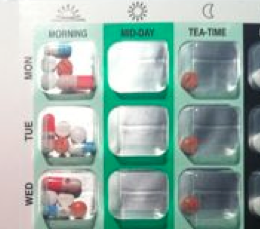
\includegraphics[scale=0.5]{agenda.png}\end{center}

	\subsection{The Systems Approach}
	With this in mind we used the systems approach to come up with a device which would perform the necessary processes to turn our inputs into the outputs we required. \bigskip \\ \includegraphics[width=\textwidth]{systems.png} \bigskip \\
	When designing a product with these specifications we had another key feature in mind: \\
	\begin{center}\emph{The patient should not have to learn anything new}.
	\end{center}
	 \medskip Ideally, they would be fed the right pills at the right time in the right dosage with no effort of their part. We wanted a solution similar to the second described above (the medical professionals) but without the cost or the inconvenience of having someone come into your home.

	\subsection{The Product}
	After looking at existing products on the market, we decided that their user interfaces were far too complex and placed too much responsibility with the patient. The image below shows a number of pill dispensing products and it can be seen that they all have a number of buttons and some of them even have small screens.
	
	\begin{center}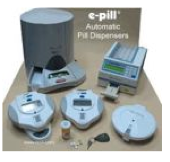
\includegraphics{pilld.png}\end{center}
	
	\begin{itemize}
	\item Simplicity: no buttons or other interaction methods. We liked the simplicity of the design of some coffee machines such as the one below, and we decided that the machine should be aesthetically pleasing, rather like most coffee machines, if the patient were to accept it as an addition to their home.
	\begin{center}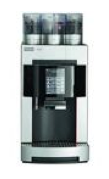
\includegraphics{coffee.png}\end{center}
	\item Safety: the pharmacist sells pre-packed tubes of medication, with a chip that the machine can read and know how much and when to dispense. No one else has access to the dosage or content of the tubes.
	\item Reliability: The machine notifies the user until it detects that the dispensed medicine is no longer in the tray. After a certain delay it notifies the nominated responsible person via telephone. The machine also notifies the pharmacist about low supplies of pills.
	\item The machine should come at a low cost to the NHS. The tubes may be refillable and reprogrammable.
	\end{itemize}
	With this in mind we sketched the physical product. These are a few attempts that focus on reduced size and a pleasant aesthetic.
	\begin{center}\includegraphics[width=0.65\textwidth]{product.png}\end{center}
	\subsubsection*{How it Works}
	\begin{enumerate}
	\item The medication is delivered by or picked up from the pharmacy where a trained person (our intermediate user) pre-packs the medicine into smart tubes. These tubes have an easily reprogrammable chip on the cap.
	\item Next the tubes are put into the machine by either the patient of the person delivering them. This is a straight forward procedure: lift the lid of the machine, place the tubes in the empty slots and close the lid.
	\item The machine reads the tubes and starts dispensing accordingly.
	\item When medicine has been dispensed the machine telephones the patient. Even if they pick up the machine will keep calling at intervals until the medicine is gone from its tray. Initially, the idea was to ask the patient to wear a bracelet or necklace that would notify the user by vibrating, however Gladys was reluctant to the idea of having to wear anything. Therefore we chose to notify the patient by an already familiar method: the telephone.
	\item After a certain time period, if the medicine has not been taken, the machine telephones a nominated person (family or doctor).
	\item The machine notifies the pharmacy via the 3G data network when it detects a low supply of medicine.
	\end{enumerate}
	
	The (poorly drawn) storyboard below shows graphically how the product would work for Gladys. \\
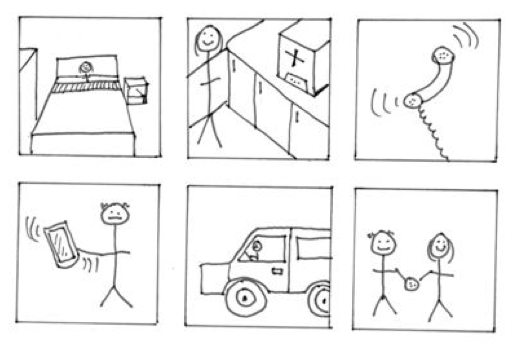
\includegraphics[width=\textwidth, angle=0.8,scale=0.95]{storyboard.png}
	\subsection{The Quantified Self}
	A useful feature of our device is that it allows the patient to remember to take their pills themself, by delaying the reminder and keeping track of how well they remember.
	\begin{itemize}
	\item Every time a patient forgets for a given time period after dispensation, the delay interval is decreased to a limit of 1 minute.
	\item Every time the patient remembers the delay is increased up to a certain upper limit.
	\end{itemize}
	The aim of this is to raise awareness and train the patient's memory. We believe these remembering patterns are an important and useful insight for the doctor to keep track of. Furthermore it gives the patient a certain independence which we found, by talking to our potential clients, is very important for their dignity at their old age. People resent the idea of being dependent on machines or other people. This system allows a modicum of self-sufficiency, whilst possibly helping them to remember their medication by themselves in future.
	
\section{Summary}
Older people have trouble remembering which medication to take, when, and how often (if at all!). Multiple solutions already exist, but they all require some degree of awareness, good memory or intervention. We have consulted real people as part of our study and reacted to feedback that they gave us about our initial designs. The system we have designed aims to obviate the need for memory and intervention, in a way so simple that anyone is able to use it without the need for a manual or instruction.

\end{document}
